%----------------------------------------------------------------------------------------
%  Monte Carlo's extimation of Pi using POSIX's pthreads	
%----------------------------------------------------------------------------------------

\section{Monte Carlo's estimation of Pi using POSIX's pthreads}

\subsection{Briefly explain the difference between a process and a thread}

A process can have multiple threads, these threads are considered within the process by the kernel.
Being a part of the same process, threads shares instruction, global, and heap region of memory.

A multi-process program has memory space for each process, hence inter-process communication is slow
because memory is not shared between them unlike threads. Context switching between process is more
expensive compared to threads - which means when the OS/Kernel switch to executing a different processes,
it has to reload the registers to regain the context for that execution, this does not happen with threads.

%------------------------------------------------

\subsection{Creating \& Joining threads using POSIX}

\Cref{lst:lab2part1a} and \cref{lst:lab2part1b} shows the creation and joining of POSIX threads.

\vspace{0.5cm}
\lstinputlisting[
	style=CStyle,
	firstline=45, % First line of code
	lastline=48, % Lastl ine of code
	caption=Creating Pthreads (line 45-48 in lab2part1.c), % Caption above the listing
	label=lst:lab2part1a, % Label for referencing this listing
	frame=single, % Frame around the code listing
	showstringspaces=false, % Don't put marks in string spaces
	numbers=left, % Line numbers on left
	numberstyle=\normalsize % Line numbers styling
	]{../code/lab2part1.c}

\vspace{0.5cm}
\lstinputlisting[
	style=CStyle,
	firstline=49, % First line of code
	lastline=51, % Lastl ine of code
	caption=Joining Pthreads (line 49-51 in lab2part1.c), % Caption above the listing
	label=lst:lab2part1b, % Label for referencing this listing
	frame=single, % Frame around the code listing
	showstringspaces=false, % Don't put marks in string spaces
	numbers=left, % Line numbers on left
	numberstyle=\normalsize % Line numbers styling
	]{../code/lab2part1.c}

%------------------------------------------------

\subsection{Generating random uniformly distributed dart tosses}

\Cref{lst:lab2part1c} shows the subroutine that generates uniformly distributed dart tosses between [-1, 1].
Each worker thread runs this subroutine, and counts the number of tosses that falls within the unit circle.

\vspace{0.5cm}
\lstinputlisting[
	style=CStyle,
	firstline=82, % First line of code
	lastline=89, % Lastl ine of code
	caption=Generating uniformly distributed dart tosses (line 82-89 in lab2part1.c), % Caption above the listing
	label=lst:lab2part1c, % Label for referencing this listing
	frame=single, % Frame around the code listing
	showstringspaces=false, % Don't put marks in string spaces
	numbers=left, % Line numbers on left
	numberstyle=\normalsize % Line numbers styling
	]{../code/lab2part1.c}

%------------------------------------------------

\subsection{Initializing and destroying Mutex}

\vspace{0.5cm}
\lstinputlisting[
	style=CStyle,
	firstline=42, % First line of code
	lastline=42, % Lastl ine of code
	caption=Initializing Mutex (line 42 in lab2part1.c), % Caption above the listing
	label=lst:lab2part1d, % Label for referencing this listing
	frame=single, % Frame around the code listing
	showstringspaces=false, % Don't put marks in string spaces
	numbers=left, % Line numbers on left
	numberstyle=\normalsize % Line numbers styling
	]{../code/lab2part1.c}

\vspace{0.5cm}
\lstinputlisting[
	style=CStyle,
	firstline=56, % First line of code
	lastline=56, % Lastl ine of code
	caption=Destroying Mutex (line 56 in lab2part1.c), % Caption above the listing
	label=lst:lab2part1e, % Label for referencing this listing
	frame=single, % Frame around the code listing
	showstringspaces=false, % Don't put marks in string spaces
	numbers=left, % Line numbers on left
	numberstyle=\normalsize % Line numbers styling
	]{../code/lab2part1.c}

%----------------------------------------------------------------------------------------

\subsection{Computing global sum of the number of dart tosses within the unit circle}

\Cref{lst:lab2part1f} shows the code that compute the global sum of all 'successful'
samples whilst avoiding any race condition using mutex.

\vspace{0.5cm}
\lstinputlisting[
	style=CStyle,
	firstline=95, % First line of code
	lastline=98, % Lastl ine of code
	caption=Computing global sum (line 95-98 in lab2part1.c), % Caption above the listing
	label=lst:lab2part1f, % Label for referencing this listing
	frame=single, % Frame around the code listing
	showstringspaces=false, % Don't put marks in string spaces
	numbers=left, % Line numbers on left
	numberstyle=\normalsize % Line numbers styling
	]{../code/lab2part1.c}

%----------------------------------------------------------------------------------------

\subsection{Results}

Estimating $\pi$ with Monte Carlo's method using $10^9$ tosses with 4 threads vs 1 thread. The linux Time
command was used to time the execution.

\begin{figure}[ht]
	\centering
	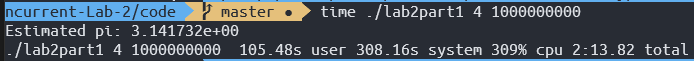
\includegraphics[width=\textwidth]{Figures/part1_4_10e9.PNG}
	\caption{Terminal output of lab2part1.c program using $10^9$ tosses with 4 threads}
	\label{fig:part1_4_10e9}
\end{figure}

\begin{figure}[ht]
	\centering
	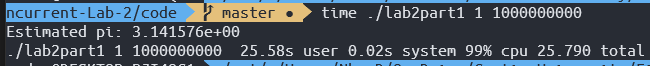
\includegraphics[width=\textwidth]{Figures/part1_1_10e9.PNG}
	\caption{Terminal output of lab2part1.c program using $10^9$ tosses with 1 threads}
	\label{fig:part1_1_10e9}
\end{figure}

The estimated values for $\pi$ was accurate to 3 decimal places. It took 2:13.82s to compute $\pi$ using
$10^9$ samples with 4 threads, and only 25.790s to compute with 1 thread per \cref{fig:part1_4_10e9} 
and \cref{fig:part1_1_10e9} respectively. 